% \date{May 14, 2024}
% \author{Deralive}
% \title{华东师范大学软件学院实验报告模板}
% 注意事项:编译两次,以确保目录、页码完整显示

\def\allfiles{}

%————————————多文件编译————————————%
% \ifx\allfiles\undefined
% 	    \begin{document}
% \else
% \fi

% Content

% \ifx\allfiles\undefined
% 	    \end{document}
% 	\else
% 	\fi
%—————————————————————————————————%

\documentclass[14pt,a4paper,UTF8,twoside]{article}

\usepackage{amsmath}
\usepackage{graphicx}
\usepackage{geometry}
\usepackage{forest}
\usepackage{ctex}
\usepackage{booktabs} % 表格库
\usepackage{titlesec} % 标题库
\usepackage{fancyhdr} % 页眉页脚库
\usepackage{lastpage} % 页码数库
\usepackage{listings} % 代码块包
\usepackage{xcolor}
\usepackage[hidelinks]{hyperref}
\usepackage{tikz}
\usepackage{tikz-qtree}
\usepackage{fontspec} % 允许设置字体
\usepackage{unicode-math} % 允许数学公式使用特定字体
\usepackage{mwe}
\usepackage{zhlipsum} % 中文乱数文本
\usepackage{amsmath}
\usepackage{xcolor}
\usepackage{float} % 浮动体环境
\usepackage{subcaption} % 子图包
\usepackage{biblatex}
\addbibresource{references.bib} % 指定你的.bib文件名称

\definecolor{mygreen}{rgb}{0,0.6,0}
\definecolor{mygray}{rgb}{0.5,0.5,0.5}
\definecolor{mymauve}{rgb}{0.58,0,0.82}

\date{} % 留空,以让编译时去除日期

%———————————————注意事项—————————————————%

% 1、如果编译显示失败,但没有错误信息,就是 filename.pdf 正在被占用
% 2、在文件夹中的终端使用 Windows > xelatex filename.tex 也可编译

%—————————————华东师范大学———————————————%

% 论文制作时须加页眉,页眉从中文摘要开始至论文末
% 偶数页码内容为:华东师范大学硕士学位论文,奇数页码内容为学位论文题目

%————————定义 \section 的标题样式————————%

% 注意:\chapter 等命令,内部使用的是 \thispagestyle{plain} 的排版格式
% 若需要自己加上页眉,实际是在用 \thispagestyle{fancy} 的排版格式
% 加上下面这一段指令,就能够让 \section 也使用 fancy 的排版格式
% 本质就是让目录、第一页也能够显示页眉、页脚

\fancypagestyle{plain}{
  \pagestyle{fancy}
}

\title{华东师范大学软件学院课程作业} % 模板
\titleformat{\section}
    {\normalfont\bfseries\Large} % 字体大小、字体系列(\bfseries 为加粗)
    {\thesection}{1em}{}

% 设置章节的中文格式
\renewcommand\thesection{\chinese{section} \hspace{0pt}}
\renewcommand\thesubsection{\arabic{subsection} \hspace{0pt}}
% \renewcommand\thesubsubsection{\alph{subsubsection} \hspace{0pt}} % 字母编号
% \hspace{0pt} 是为了确保在章节编号和章节题目之间不要有空格,使得排版更为美观
    
%—————————————页面基础设置———————————————%

\geometry{left=10mm, right=10mm, top=20mm, bottom=20mm}

%————————————设置页眉、页脚——————————————%

\pagestyle{fancy} % 设置 plain style 的属性

% 设置页眉

\fancyhead[RE]{\leftmark} % Right Even 偶数页右侧显示章名 \leftmark 最高级别章名
\fancyhead[LO]{\rightmark} % Left Odd 奇数页左侧显示节名 \rightmark 第二级别节名
\fancyhead[C]{华东师范大学软件学院课程作业} % Center 居中显示
\fancyhead[LE,RO]{~\thepage~} % 在偶数页的左侧,奇数页的右侧显示页码
\renewcommand{\headrulewidth}{1.2pt} % 页眉与正文之间的水平线粗细

% 设置页脚:在每页的右下脚以斜体显示书名

\fancyfoot[RO,RE]{\it Lab Report By \LaTeX} % 使用意大利斜体显示
\renewcommand{\footrulewidth}{0.5pt} % 页脚水平线宽度

% 设置页码:在底部居中显示页码

\pagestyle{fancy}
\fancyfoot[C]{\kaishu 第 \thepage 页 \ 共 \pageref{LastPage} 页} % LastPage 需要二次编译以获取总页数

%——————————————代码块设置———————————————%

\lstset {
    backgroundcolor=\color{white},   % choose the background color; you must add \usepackage{color} or \usepackage{xcolor}
    basicstyle=\footnotesize,        % the size of the fonts that are used for the code
    breakatwhitespace=false,         % sets if automatic breaks should only happen at whitespace
    breaklines=true,                 % sets automatic line breaking
    captionpos=bl,                   % sets the caption-position to bottom
    commentstyle=\color{mygreen},    % comment style
    deletekeywords={...},            % if you want to delete keywords from the given language
    escapeinside={\%*}{*},           % if you want to add LaTeX within your code
    extendedchars=true,              % lets you use non-ASCII characters; for 8-bits encodings only, does not work with UTF-8
    frame=single,                    % adds a frame around the code
    keepspaces=true,                 % keeps spaces in text, useful for keeping indentation of code (possibly needs columns=flexible)
    keywordstyle=\color{blue},       % keyword style
    % language=Python,               % the language of the code
    morekeywords={*,...},            % if you want to add more keywords to the set
    numbers=left,                    % where to put the line-numbers; possible values are (none, left, right)
    numbersep=5pt,                   % how far the line-numbers are from the code
    numberstyle=\tiny\color{mygray}, % the style that is used for the line-numbers
    rulecolor=\color{black},         % if not set, the frame-color may be changed on line-breaks within not-black text (e.g. comments (green here))
    showspaces=false,                % show spaces everywhere adding particular underscores; it overrides 'showstringspaces'
    showstringspaces=false,          % underline spaces within strings only
    showtabs=false,                  % show tabs within strings adding particular underscores
    stepnumber=1,                    % the step between two line-numbers. If it's 1, each line will be numbered
    stringstyle=\color{orange},      % string literal style
    tabsize=2,                       % sets default tabsize to 2 spaces
    % title=Python Code              % show the filename of files included with \lstinputlisting; also try caption instead of title
}

% 注释掉的部分用于后续插入代码,参数可调整,格式如下:

% 1、直接插入
% \begin{lstlisting}[language = ? , title = { ? } ]
%       Your code here.
% \end{lstlisting}

% 2、文件插入
% \lstinputlisting[language = C , title = ?.c] {filename.c}

%———————————————字体设置————————————————%

% \setCJKmainfont{SimSun} % 设置正文罗马族的 CJK 字体
% \renewcommand{\normalsize}{\fontsize{12pt}{15pt}\selectfont} % 设置正文字号
\linespread{1.2}

%——————————————————————————————————————%

%———————————————超链接设置——————————————%

\hypersetup{
    pdfstartview=FitH, % 设置PDF文档打开时的初始视图为页面宽度适应窗口宽度(即页面水平适应)
    CJKbookmarks=true, % 用对CJK(中文、日文、韩文)字符的书签支持,确保这些字符在书签中正确显示
    bookmarksnumbered=true, % 书签带有章节编号。这对有章节编号的文档很有用
    bookmarksopen=true, % 文档打开时,书签树是展开的,方便查看所有书签
    colorlinks, % 启用彩色链接。这样,链接在PDF中会显示为彩色,而不是默认的方框
    pdfborder=001, % 设置PDF文档中链接的边框样式。001 表示链接周围没有边框,仅在单击时显示一个矩形
    linkcolor=blue, % 设置文档内部链接(如目录中的章节链接)的颜色为蓝色
    anchorcolor=blue, % 设置锚点链接(即目标在同一文档内的链接)的颜色为蓝色
    citecolor=blue, % 设置引用(如文献引用)的颜色为蓝色
}

%——————————————导言区结束,进入正文部分———————————————%

%——————————————————————————————————————%

\begin{document}

\maketitle

\begin{center} % \extracolsep{\fill} 拉伸到页面最大宽度前,保证居中显示

  \begin{tabular*}{\textwidth}{@{\extracolsep{\fill}} l  l  l }
    \hline
    课程名称:计算机网络 &  年级:2023级本科  &  姓名:张梓卫 \\
    作业主题:第五章作业 & 学号:10235101526 & 作业日期:2024/12/16 \\
    指导老师:刘献忠 & 组号: \\
    \hline
  \end{tabular*}

\end{center}

% \tableofcontents % 目录也需要二次编译

\section{5.1}

\subsection*{题目}
Consider the network of Fig.5-7, but ignore the weights on the lines. Suppose that it uses flooding as the routing algorithm. If a packet sent by A to D has a maximum hop count of 3, list all the routes it will take. Also tell how many hops worth of bandwidth it consumes.

考虑图 Fig.5-7 的网络,忽略线上的权重。假设它使用洪泛作为路由算法。

如果 A 发送到 D 的数据包最大跳数为 3,列出它将采取的所有路由。还要说明它消耗了多少跳数的带宽。

\subsection*{解答}

\begin{figure}[H]
  \centering
  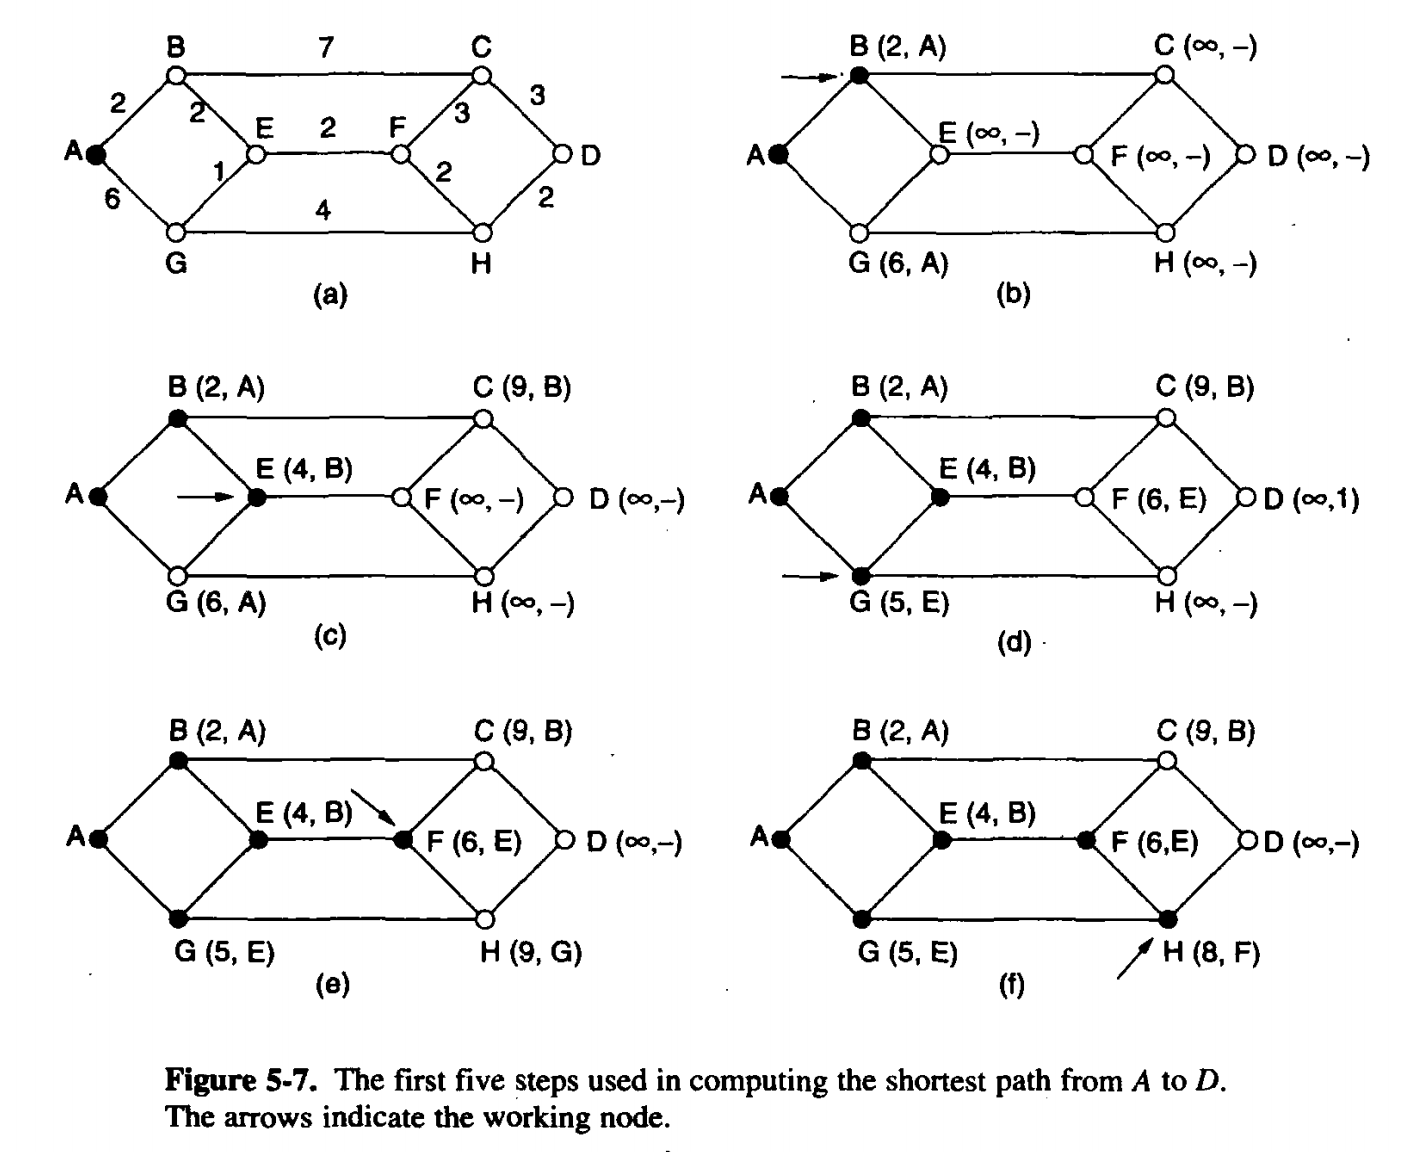
\includegraphics[width=0.5\textwidth]{lec5/5-7.png}
  \caption{Fig.5-7}
\end{figure}

根据洪泛法的传播规则,每个节点会将数据包发送到所有相邻节点,除了数据包刚来的那条路径。在 最大跳数 = 3 的限制下,从起点 A 开始传播,所有到达 D 的路径为:

\begin{center}
  \begin{forest}
    for tree={%
    grow'=270,           % 树向下生长
    parent anchor=south,% 父节点的锚点在下方
    child anchor=north, % 子节点的锚点在上方
    l sep=8pt,         % 节点水平间隔
    s sep=12pt,         % 节点垂直间隔
    thick,              % 线条加粗
    edge={thick, draw, ->}, % 强制绘制线条并加粗
    align=center        % 节点内容居中
},
  [A
    [B
      [C
        [D]
        [F]
      ]
      [E
        [F]
        [G]
      ]
    ]
    [G
      [H
        [D]
        [F]
      ]
      [E
        [F]
        [B]
      ]
    ]
  ]
  \end{forest}
\end{center}

\section*{路径列表}

以下是从节点 \textbf{A} 到 \textbf{D} 的所有路径:

\begin{itemize}
    \item \(\textbf{A} \rightarrow \textbf{B} \rightarrow \textbf{C} \rightarrow \textbf{D}\), \(\textbf{A} \rightarrow \textbf{B} \rightarrow \textbf{C} \rightarrow \textbf{F}\), \(\textbf{A} \rightarrow \textbf{B} \rightarrow \textbf{E} \rightarrow \textbf{F}\), \(\textbf{A} \rightarrow \textbf{B} \rightarrow \textbf{E} \rightarrow \textbf{G}\)
    \item \(\textbf{A} \rightarrow \textbf{G} \rightarrow \textbf{H} \rightarrow \textbf{D}\),  \(\textbf{A} \rightarrow \textbf{G} \rightarrow \textbf{H} \rightarrow \textbf{F}\),  \(\textbf{A} \rightarrow \textbf{G} \rightarrow \textbf{E} \rightarrow \textbf{F}\),  \(\textbf{A} \rightarrow \textbf{G} \rightarrow \textbf{E} \rightarrow \textbf{B}\)
\end{itemize}

观察该树状结构,可以看出共有 14 条边,即消耗了 14 跳的带宽。

\section{5.2}

\subsection*{题目}
Consider the network of Fig. 5-13(a). Distance vector routing is used, and the following vectors have just come in to router C: from B: (5, 0, 8, 12, 6, 2); from D: (16, 12, 6, 0, 9, 10); and from E: (7, 6, 3, 9, 0, 4). The cost of the links from C to B, D, and E, are 6, 3, and 5, respectively. What is C’s new routing table? Give both the outgoing line to use and the cost.

考虑图 Fig.5-13(a) 的网络。使用距离矢量路由,以下矢量刚刚传递到路由器 C:从 B: (5, 0, 8, 12, 6, 2);从 D: (16, 12, 6, 0, 9, 10);从 E: (7, 6, 3, 9, 0, 4)。从 C 到 B、D 和 E 的链路成本分别是 6、3 和 5。C 的新路由表是什么?请同时给出出站线路的名称和成本。

\subsection*{解答}

每个路由器通过邻居的距离向量表更新自己的路由表,选择成本最低的路径进行转发。

\begin{figure}[H]
  \centering
  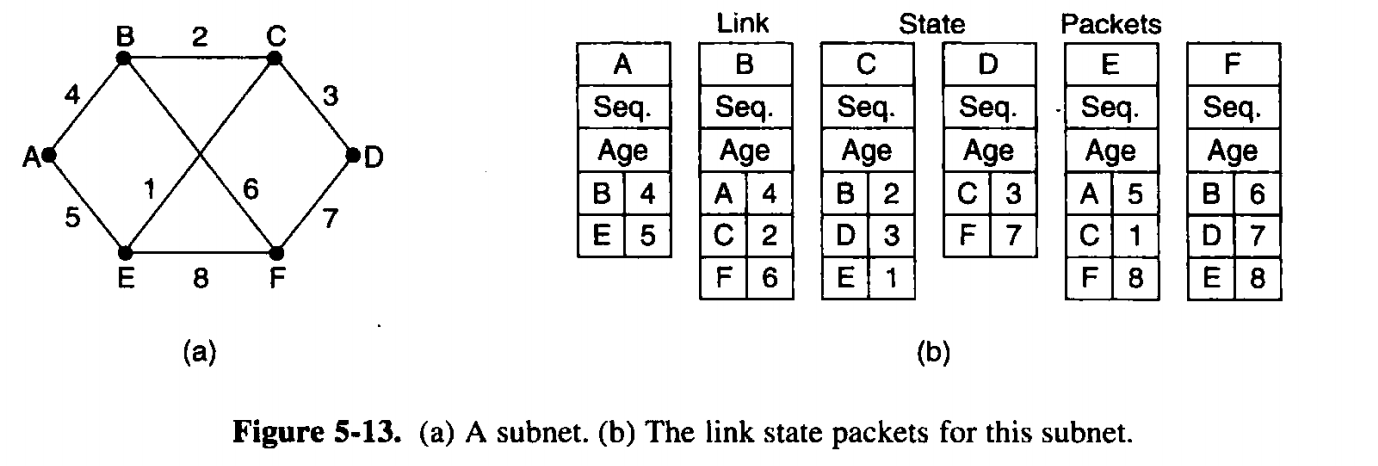
\includegraphics[width=0.5\textwidth]{lec5/5-13.png}
  \caption{Fig.5-13(a)}
\end{figure}

对于每个邻居B, D, E,我们将 C 到邻居的成本 加上 邻居到各目标的成本。

\begin{itemize}
  \item 由于 $ C \rightarrow B = 6 $ , 通过 B 给出 (11, 6, 14, 18, 12, 8). 
  \item 通过 $ D \rightarrow B = 3 $ , 通过 D 给出 (19, 15, 9, 3, 12, 13). 
  \item 通过 $ E \rightarrow B = 5 $ , 通过 E 给出 (12, 11, 8, 14, 5, 9).
\end{itemize}

\begin{table}[H]
  \centering
  \renewcommand{\arraystretch}{1.2} % 调整表格的行高
  \begin{tabular}{|l|c|c|c|c|c|c|} 
  \hline
  \textbf{}          & \textbf{A} & \textbf{B} & \textbf{C} & \textbf{D} & \textbf{E} & \textbf{F} \\ \hline
  \textbf{通过 B}   & 11         & 6          & -          & 18         & 12         & 8          \\ \hline
  \textbf{通过 D}   & 19         & 15         & -          & 3          & 12         & 13         \\ \hline
  \textbf{通过 E}   & 12         & 11         & -          & 14         & 5          & 9          \\ \hline
  \textbf{最小成本} & 11         & 6          & 0          & 3          & 5          & 8          \\ \hline
  \textbf{下一跳}   & B          & B          & -          & D          & E          & B          \\ \hline
  \end{tabular}
  \caption{C 的路由表}
  \label{tab:reverse_routing_table}
\end{table}

取除 C 以外的每个目的地的最小值,可以得到 (11, 6, 0, 3, 5, 8). 

所以输出线路即为:(B, B,– , D, E, B).

\section{5.3}

\subsection*{题目}
Looking at the network of Fig. 5-6, how many packets are generated by a broadcast from B, using 

(a) Reverse path forwarding?

(b) The sink tree?

观察图 Fig.5-6 的网络,从 B 开始进行广播,生成多少个数据包:

(a) 使用反向路径转发?

(b) 使用汇聚树?

\subsection*{解答}

\begin{figure}[H]
  \centering
  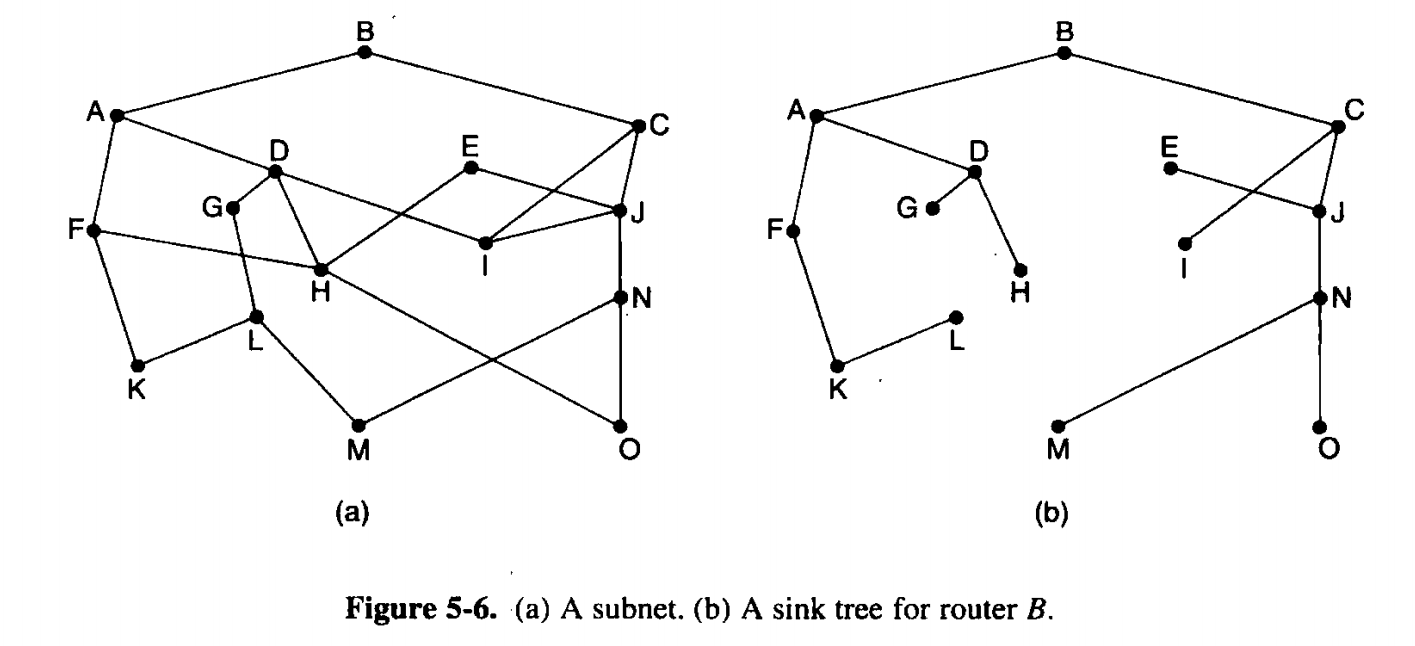
\includegraphics[width=0.5\textwidth]{lec5/5-6.png}
  \caption{Fig.5-6}
\end{figure}

\subsection*{(a) 使用反向路径转发:}

反向路径转发是一种防止广播风暴的方法。其核心规则是:

每个节点接收到数据包后,只会将数据包转发给其他相邻节点(除了刚接收到数据包的节点)。

同一个节点接收到的数据包会被过滤,确保不会重复传播。

\begin{center}
  \begin{forest}
  for tree={%
      grow'=270,            % 树向下生长
      parent anchor=south,  % 父节点的锚点在下方
      child anchor=north,   % 子节点的锚点在上方
      l sep=8pt,           % 水平间隔
      s sep=12pt,           % 垂直间隔
      thick,                % 线条加粗
      edge={thick, draw, ->}, % 使用带箭头的线条
      align=center          % 节点内容居中
  }
  [B
      [C
          [J
              [N
                  [O
                      [H]
                  ]
                  [M
                      [L]
                  ]
              ]
              [I]
              [E
                [H]
              ]
          ]
          [I
              [J]
              [D]
          ]
      ]
      [A
          [D
              [I]
              [H]
              [G
                  [L]
              ]
          ]
          [F
            [H
              [O]
              [E]
              [D]
            ]
            [K
              [L
                [G]
                [M]
              ]
            ]
          ]
      ]
  ]
  \end{forest}
\end{center}

共有 $ 2 + 4 + 10 + 8 + 4 = 28 $ 个数据包。

\vspace{0.5cm}

\subsection*{(b) 使用汇聚树:}

汇聚树是一棵以源节点为根的树,从根出发,到达网络中所有节点的最短路径。

在这种情况下,每个节点只接收一次数据包,因为树结构中没有环路。

\begin{center}
  \begin{forest}
  for tree={%
      grow'=270,            % 树向下生长
      parent anchor=south,  % 父节点锚点在下方
      child anchor=north,   % 子节点锚点在上方
      l sep=20pt,           % 水平间隔
      s sep=20pt,           % 垂直间隔
      thick,                % 线条加粗
      edge={thick, draw, ->}, % 使用带箭头的线条
      align=center          % 节点内容居中
  }
  [B
      [A
          [F
              [K
                  [L]
              ]
          ]
          [D
              [G]
              [H]
          ]
      ]
      [C
          [I]
          [J
              [E]
              [N
                  [O]
                  [M]
              ]
          ]
      ]
  ]
  \end{forest}
\end{center}

共有 $ 2 + 4 + 5 + 3 = 14 $ 个数据包。

\section{5.4}

\subsection*{题目}
Suppose that host A is connected to a router R 1, R 1 is connected to another router, R 2, and R 2 is connected to host B. Suppose that a TCP message that contains 900 bytes of data and 20 bytes of TCP header is passed to the IP code at host A for delivery to B. Show the Total length, Identification, DF, MF, and Fragment offset fields of the IP header in each packet transmitted over the three links. Assume that link A-R1 can support a maximum frame size of 1024 bytes including a 14-byte frame header, link R1-R2 can support a maximum frame size of 512 bytes, including an 8-byte frame header, and link R2-B can support a maximum frame size of 512 bytes including a 12-byte frame header.

假设主机 A 连接到路由器 R1,R1 连接到另一个路由器 R2,R2 连接到主机 B。假设一条包含 900 字节数据和 20 字节 TCP 头的数据包被传递给 IP 层,在这三个链路上传输时显示 IP 包的总长度、Identification、DF、MF 和 Fragment Offset 字段的内容。假设链路 A-R1 可以支持 1024 字节的最大帧大小(包括 14 字节帧头),链路 R1-R2 的最大帧大小是 512 字节(包括 8 字节帧头),链路 R2-B 的最大帧大小是 512 字节(包括 12 字节帧头)。

\subsection*{解答}

\noindent \textbf{\large A————R1————R2————B} \\

不妨设 IPV4 协议头为 20 字节。

A——R1: 最大帧大小 = 1024B,包括 14B 的帧头
最大 IP 数据包大小 = 1024B - 14B = 1010B。

R1——R2: 最大帧大小 = 512B,包括 8B 的帧头
最大 IP 数据包大小 = 512B - 8B = 504B。

R2——B: 最大帧大小 = 512B,包括 12B 的帧头
最大 IP 数据包大小 = 512B - 12B = 500B。

\textbf{IP Packet(20B+920B)} \\[5pt]

\begin{center}
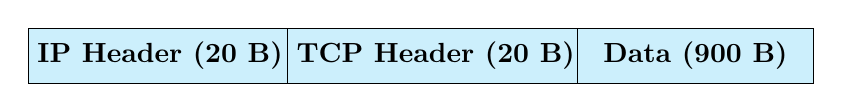
\begin{tikzpicture}
% 第1行:IP头、TCP头、数据
\node[draw, fill=cyan!20, minimum width=3cm, minimum height=0.7cm] at (0,0) {\textbf{IP Header (20 B)}};
\node[draw, fill=cyan!20, minimum width=3cm, minimum height=0.7cm] at (3.5,0) {\textbf{TCP Header (20 B)}};
\node[draw, fill=cyan!20, minimum width=3cm, minimum height=0.7cm] at (6.8,0) {\textbf{Data (900 B)}};
\end{tikzpicture}
\end{center}

\vspace{10pt}
\noindent \textbf{A————R1: 940 < 1010, 因此不需要分片} \\[5pt]

\begin{center}
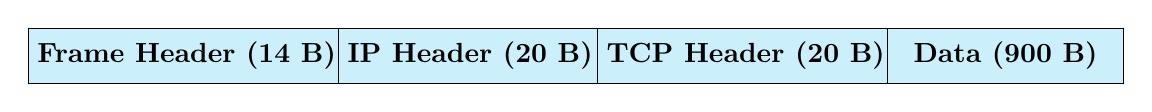
\begin{tikzpicture}
% 第2行:Frame头、IP头、TCP头、数据
\node[draw, fill=cyan!20, minimum width=1.5cm, minimum height=0.7cm] at (0,0) {\textbf{Frame Header (14 B)}};
\node[draw, fill=cyan!20, minimum width=1.5cm, minimum height=0.7cm] at (3.6,0) {\textbf{IP Header (20 B)}};
\node[draw, fill=cyan!20, minimum width=1.5cm, minimum height=0.7cm] at (7.1,0) {\textbf{TCP Header (20 B)}};
\node[draw, fill=cyan!20, minimum width=3.0cm, minimum height=0.7cm] at (10.4,0) {\textbf{Data (900 B)}};
\end{tikzpicture}
\end{center}

\vspace{10pt}
\noindent \textbf{R1————R2: 940 > 504, 需要分片, $\frac{504 - 20}{8} = 60 ... 4$} \\

IP 头占用 20B,剩余数据大小 = 504B - 20B = 484B。

IP 数据必须按 8 字节对齐,因此可传输的数据为 480B(因为 484B 向下取整到 8 的倍数)。

数据 900B 需要分两部分传输:

\begin{itemize}
  \item 第一片:480B 数据 + 20B IP 头 → 总大小 = 500B
  \item 第二片:剩余数据 = 900B - 480B = 420B
\end{itemize}
由于 420B 也需要 8 字节对齐,所以取 440B,再加上 IP 头 20B → 总大小 = 460B。


\noindent \textbf{IP Packet 1}

\begin{center}
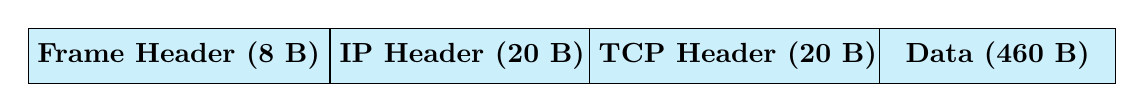
\begin{tikzpicture}
% 第3行:分片1
\node[draw, fill=cyan!20, minimum width=1.5cm, minimum height=0.7cm] at (0,0) {\textbf{Frame Header (8 B)}};
\node[draw, fill=cyan!20, minimum width=1.5cm, minimum height=0.7cm] at (3.6,0) {\textbf{IP Header (20 B)}};
\node[draw, fill=cyan!20, minimum width=1.5cm, minimum height=0.7cm] at (7.1,0) {\textbf{TCP Header (20 B)}};
\node[draw, fill=cyan!20, minimum width=3.0cm, minimum height=0.7cm] at (10.4,0) {\textbf{Data (460 B)}};
\end{tikzpicture}
\end{center}

\noindent \textbf{IP Packet 2}

\begin{center}
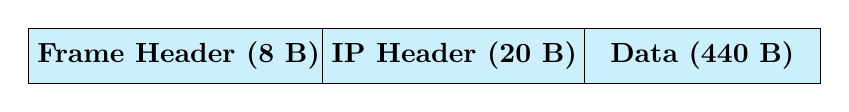
\begin{tikzpicture}
% 第4行:分片2
\node[draw, fill=cyan!20, minimum width=1.5cm, minimum height=0.7cm] at (0,0) {\textbf{Frame Header (8 B)}};
\node[draw, fill=cyan!20, minimum width=1.5cm, minimum height=0.7cm] at (3.5,0) {\textbf{IP Header (20 B)}};
\node[draw, fill=cyan!20, minimum width=3.0cm, minimum height=0.7cm] at (6.65,0) {\textbf{Data (440 B)}};
\end{tikzpicture}
\end{center}

\vspace{10pt}
\noindent \textbf{R2————B: 500 = 500, 无需分片} \\

\noindent \textbf{IP Packet 1}

\begin{center}
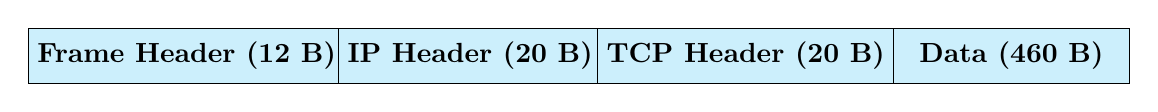
\begin{tikzpicture}
% 第5行:R2-B分片1
\node[draw, fill=cyan!20, minimum width=1.5cm, minimum height=0.7cm] at (0,0) {\textbf{Frame Header (12 B)}};
\node[draw, fill=cyan!20, minimum width=1.5cm, minimum height=0.7cm] at (3.6,0) {\textbf{IP Header (20 B)}};
\node[draw, fill=cyan!20, minimum width=1.5cm, minimum height=0.7cm] at (7.1,0) {\textbf{TCP Header (20 B)}};
\node[draw, fill=cyan!20, minimum width=3.0cm, minimum height=0.7cm] at (10.475,0) {\textbf{Data (460 B)}};
\end{tikzpicture}
\end{center}

\noindent \textbf{IP Packet 2}

\begin{center}
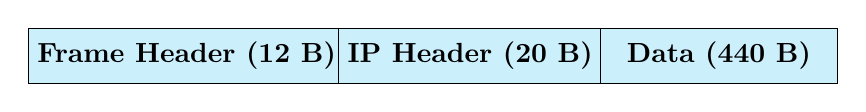
\begin{tikzpicture}
% 第6行:R2-B分片2
\node[draw, fill=cyan!20, minimum width=1.5cm, minimum height=0.7cm] at (0,0) {\textbf{Frame Header (12 B)}};
\node[draw, fill=cyan!20, minimum width=1.5cm, minimum height=0.7cm] at (3.6,0) {\textbf{IP Header (20 B)}};
\node[draw, fill=cyan!20, minimum width=3.0cm, minimum height=0.7cm] at (6.76,0) {\textbf{Data (440 B)}};
\end{tikzpicture}
\end{center}

\begin{table}[H]
  \centering
  \begin{tabular}{|c|c|c|c|c|c|}
  \hline
  \textbf{Link} & \textbf{Length} & \textbf{ID} & \textbf{DF} & \textbf{MF} & \textbf{Offset} \\ \hline
  A-R1       & 940      & x  & 0  & 0  & 0   \\ \hline
  R1-R2      & 500      & x  & 0  & 1  & 0   \\ \hline
  R1-R2      & 460      & x  & 0  & 0  & 60  \\ \hline
  R2-B       & 500      & x  & 0  & 1  & 0   \\ \hline
  R2-B       & 460      & x  & 0  & 0  & 60  \\ \hline
  \end{tabular}
  \caption{Summary of Fragmentation Fields for IP Packets}
  \label{tab:fragmentation}
\end{table}

\section{5.5}

\subsection*{题目}
A router is blasting out IP packets whose total length (data plus header) is 1024 bytes. Assuming that packets live for 10 sec, what is the maximum line speed the router can operate at without danger of cycling through the IP datagram ID number space?

一个路由器正在发送总长度为 1024 字节(数据加头部)的 IP 包。假设包的生命周期为 10 秒,那么路由器能够以多快的线路速度运行,而不会导致 IP 数据包 ID 编号空间的耗尽?

\subsection*{解答}

IP 报头标识为 16 位, 因此可以存储的最大值是 $ 2^{16} =65,535$ 个不同的 ID。

\begin{itemize}
  \item \textbf{最多可发送的数据包个数}:  
  由于标识符最多为 $2^{16} = 65,536$,因此在 10 秒内最多发送 $65,536$ 个数据包。
  
  \item \textbf{每个数据包的大小}:  
  每个 IP 包大小为 $1024 \ \text{bytes}$。
\end{itemize}

  \[
    \text{总数据量} = 65,536 \times 1024 \ \text{bytes} = 2^{16} \times 2^{10} = 2^{26} \ \text{bytes}.
  \]

  \[
    \text{总比特数} = 2^{26} \times 8 = 2^{29} \ \text{bits}.
  \]

将 $2^{29} = 536,870,912$,带入计算:
\[
b = \frac{536,870,912 \ \text{bits}}{10 \ \text{s}} = 53,687,091.2 \ \text{bps}.
\]

\begin{itemize}
    \item \textbf{最大线路速度} $b$:$53,687,091.2 \ \text{bps}$(比特每秒)。
    \item \textbf{简化单位}:大约为 \textbf{53.7 Mbps}(兆比特每秒)。
\end{itemize}

\section{5.6}

\subsection*{题目}
An IP datagram using the Strict source routing option has to be fragmented. Do you think the option is copied into each fragment, or is it sufficient to just put it in the first fragment? Explain your answer.

严格源路由选项需要被分段。你认为这个选项是否需要复制到每个分段中,还是仅放在第一个分段中即可?

请解释你的答案。

\subsection*{解答}

严格源路由选项(Strict Source Routing Option)需要被复制到每个分片中,因为接收方以及中间路由器需要严格遵循源指定的路由规则来处理这些数据包的每一个分片。如果仅将选项放在第一个分片中,则后续分片在路由过程中会丢失关键信息,导致路由失败或行为异常。

严格源路由选项是路由过程中必不可少的信息,每个分片在经过中间路由器时都需要参考该选项来确定下一跳。
如果该选项未被复制到某些分片中,这些分片可能无法按照指定路径到达目的地,导致数据包传输失败。

接收方在组装分片时也需要知道这些分片来自严格源路由的包,从而在必要情况下向源地址反馈问题。

\section{5.7}

\subsection*{题目}
Suppose that instead of using 16 bits for the network part of a class B address originally, 20 bits had been used. How many class B networks would there have been?

假设在最初使用类 B 地址时,网络部分使用的是 16 位,而现在改为 20 位,那么会有多少个类 B 网络?

\subsection*{解答}

类 B 地址的特点如下:
\begin{itemize}
    \item IP 地址总共 \( 32 \) 位。
    \item 类 B 地址的前 \( 2 \) 位固定为 \( 10 \)。
\end{itemize}

如果网络部分使用 \( 20 \) 位,其中前 \( 2 \) 位固定为 \( 10 \),那么剩余的位数是:
\[
20 - 2 = 18 \ \text{位}.
\]

因此,网络部分可以表示的网络数量为:
\[
2^{18} = 262,144.
\]

然而,全 \( 0 \) 和全 \( 1 \) 的地址是特殊地址,不能用作网络地址。因此,可用的网络数量为:
\[
2^{18} - 2 = 262,142 \ \text{个}.
\]

\section{5.8}

\subsection*{题目}
A network on the Internet has a subnet mask of 255.255.240.0. What is the maximum number of hosts it can handle?

互联网中的一个网络具有子网掩码 255.255.240.0。它能容纳的最大主机数是多少?

\subsection*{解答}

子网掩码 \( 255.255.240.0 \) 的二进制形式为:
\[
11111111.11111111.11110000.00000000
\]

\noindent 其中:
\begin{itemize}
    \item 连续的 \( 1 \) 表示网络部分,共 \( 20 \) 位。连续的 \( 0 \) 表示主机部分,共 \( 12 \) 位。
\end{itemize}

主机部分的位数为 \( 12 \),因此主机地址的总数为:$2^{12} = 4096$。

然而要记住,有两个地址不能使用:
\begin{itemize}
    \item 全 \( 0 \):网络地址;全 \( 1 \):广播地址。
\end{itemize}

因此,可用的主机数为:
\[
2^{12} - 2 = 4096 - 2 = 4094
\]

\section{5.9}

\subsection*{题目}
A large number of consecutive IP addresses are available starting at 198.16.0.0. Suppose that four organizations, A, B, C, and D, request 4000, 2000, 4000, and 8000 addresses, respectively, and in that order. For each of these, give the first IP address assigned, the last IP address assigned, and the mask in the w.x.y.z/s notation.

从 198.16.0.0 开始的一大块连续 IP 地址分配。假设四个组织 A、B、C 和 D 分别请求 4000、2000、4000 和 8000 个地址。对于每个组织,给出分配的第一个 IP 地址、最后一个 IP 地址以及子网掩码。

\subsection*{解答}

根据题目要求,将请求的地址数量向上取整到 2 的幂次方,并依次分配地址块。

\noindent \textbf{计算过程}:
\begin{itemize}
  \item 请求的地址数量向上取整到 2 的幂次方:
  \item 
  \( 4000 \to 2^{12} = 4096 \),\( 2000 \to 2^{11} = 2048 \),\( 4000 \to 2^{12} = 4096 \),\( 8000 \to 2^{13} = 8192 \)。
  \item 从 198.16.0.0 开始,依次分配地址块,计算每个组织的起始和结束地址。
\end{itemize}

\begin{itemize}
  \item \textbf{起始地址}:\( 198.16.0.0 \) 的二进制表示为:
  \[
  11000110.00010000.00000000.00000000
  \]
  \item \textbf{最后一个地址}:低 12 位全为 1,高 20 位保持不变,得到:
  \[
  11000110.00010000.00001111.11111111
  \]
  将其转换为十进制,得到 \( 198.16.15.255 \)。
\end{itemize}

\noindent \textbf{地址范围}:  
\[
198.16.0.0 \ \text{到} \ 198.16.15.255
\]

\noindent \textbf{子网掩码 /20}:表示前 20 位为网络位,主机位为 12 位,可容纳 \( 2^{12} = 4096 \) 个地址。

后续的也按照相同的方法,可以得到以下的表格结果:

\begin{table}[H]
  \centering
  \renewcommand{\arraystretch}{1.2}
  \begin{tabular}{|c|l|l|c|c|}
    \hline
    \textbf{组织} & \textbf{起始地址} & \textbf{结束地址} & \textbf{地址块大小} & \textbf{子网掩码} \\ \hline
    A   & 198.16.0.0    & 198.16.15.255   & 4096  & /20 \\ \hline
    B   & 198.16.16.0   & 198.16.23.255   & 2048  & /21 \\ \hline
    C   & 198.16.32.0   & 198.16.47.255   & 4096  & /20 \\ \hline
    D   & 198.16.64.0   & 198.16.95.255   & 8192  & /19 \\ \hline
  \end{tabular}
  \caption{IP 地址分配及子网掩码}
  \label{tab:ip_allocation}
\end{table}

\section{5.10}

\subsection*{题目}
A router has the following (CIDR) entries in its routing table:

一个路由器具有以下 (CIDR) 路由表:

\begin{table}[H]
    \centering
    \begin{tabular}{|l|l|}
        \hline
        \textbf{Address/Mask} & \textbf{Next Hop}     \\ \hline
        135.46.56.0/21   & Interface 0        \\ \hline
        135.46.48.0/20   & Interface 1        \\ \hline
        192.53.40.0/23   & Router 1        \\ \hline
        Default          & Router 2        \\ \hline
    \end{tabular}
\end{table}

\vspace{1cm}

For each of the following IP addresses, what does the router do if a packet with that
address arrives?

对于下面的每个IP地址,如果一个数据包带有该IP地址,路由器会做什么?

(a) 135.46.63.10

(b) 135.46.57.14

(c) 135.46.52.2

(d) 192.53.40.7

(e) 192.53.56.7

\subsection*{解答}

CIDR(无类域间路由)中IP地址和子网掩码的匹配规则。路由器的工作是基于最长匹配原则,即匹配的网络前缀越长(掩码越小),路由器会选择该路由表项转发数据包。

\section*{解答步骤}

1. 对每个 IP 地址取出第三字节,将其转换为二进制。

2. 根据路由表的地址前缀匹配,找到最长匹配的路由表项。

3. 若无匹配项,使用默认路由。

\section*{路由表项}

\begin{center}
\begin{tabular}{|l|l|l|}
\hline
\textbf{Address/mask} & \textbf{第三字节 (二进制)} & \textbf{Next Hop} \\ \hline
135.46.56.0/22 & 0011 1000 & Interface 0 \\ \hline
135.46.60.0/22 & 0011 1100 & Interface 1 \\ \hline
192.53.40.0/23 & 0010 1000 & Router 1 \\ \hline
default & - & Router 2 \\ \hline
\end{tabular}
\end{center}

根据最长前缀匹配原则,结果如下:

\section*{每个目标 IP 地址与路由表匹配过程}

\begin{enumerate}
    \item \textbf{(a) 135.46.63.10}  
    \begin{itemize}
        \item \textbf{第三字节}:63 转换为二进制:\texttt{0011 1111}
        \item 匹配的最长前缀是 \texttt{135.46.60.0/22}(\texttt{0011 11xx} 匹配)
        \item \textbf{Next hop}:\textbf{Interface 1}
    \end{itemize}

    \item \textbf{(b) 135.46.57.14}  
    \begin{itemize}
        \item \textbf{第三字节}:57 转换为二进制:\texttt{0011 1001}
        \item 匹配的最长前缀是 \texttt{135.46.56.0/22}(\texttt{0011 10xx} 匹配)
        \item \textbf{Next hop}:\textbf{Interface 0}
    \end{itemize}

    \item \textbf{(c) 135.46.52.2}  
    \begin{itemize}
        \item \textbf{第三字节}:52 转换为二进制:\texttt{0011 0100}
        \item 没有与前缀 \texttt{135.46.56.0/22} 或 \texttt{135.46.60.0/22} 匹配。
        \item 使用默认路由:\textbf{Router 2}
    \end{itemize}

    \item \textbf{(d) 192.53.40.7}  
    \begin{itemize}
        \item \textbf{第三字节}:40 转换为二进制:\texttt{0010 1000}
        \item 匹配的最长前缀是 \texttt{192.53.40.0/23}(\texttt{0010 10xx} 匹配)
        \item \textbf{Next hop}:\textbf{Router 1}
    \end{itemize}

    \item \textbf{(e) 192.53.56.7}  
    \begin{itemize}
        \item \textbf{第三字节}:56 转换为二进制:\texttt{0011 1000}
        \item 没有匹配的前缀(\texttt{192.53.40.0/23} 不匹配)。
        \item 使用默认路由:\textbf{Router 2}
    \end{itemize}
\end{enumerate}

获得最终总结的内容如下表所示:

\begin{table}[H]
  \centering
  \renewcommand{\arraystretch}{1.3}
  \setlength{\tabcolsep}{12pt}
  \begin{tabular}{|c|c|c|c|}
      \hline
      \textbf{No.} & \textbf{Destination IP Address} & \textbf{The 3\textsuperscript{rd} Byte (in Binary)} & \textbf{Output} \\ \hline
      \textbf{(a)} & 135.46.63.10 & 0011 1111 & Interface 1 \\ \hline
      \textbf{(b)} & 135.46.57.14 & 0011 1001 & Interface 0 \\ \hline
      \textbf{(c)} & 135.46.52.2  & 0011 0100 & Router 2 \\ \hline
      \textbf{(d)} & 192.53.40.7  & 0010 1000 & Router 1 \\ \hline
      \textbf{(e)} & 192.53.56.7  & 0011 1000 & Router 2 \\ \hline
  \end{tabular}
  \caption{Destination IP Address and Matching Output}
\end{table}

\end{document}